\documentclass[12pt]{article}
\usepackage[a4paper]{geometry}
\usepackage[pdftex]{hyperref}
\usepackage[german]{babel}
\usepackage[utf8]{inputenc}
\usepackage{csquotes}
\usepackage{amssymb}
\usepackage{graphicx}
\usepackage{multicol}
\usepackage{amsmath}
\usepackage{enumitem}
\usepackage{fancyhdr}
\usepackage{indentfirst}
\usepackage{polynom}

\geometry{
  headheight=14px,
  left=2.54cm,
  right=2.54cm,
  bottom=2cm,
  top=2cm
}

\setlength{\marginparsep}{1 cm}
\setlength{\topmargin}{-0.6in}
\setlength{\textheight}{9.5in}
\pagestyle{fancy}

% German-style quotation marks %
\MakeOuterQuote{"}

% Typesetting differential operator %
\providecommand\d{}
\renewcommand{\d}[1]{\:\mathrm{d}{#1}} 

\polyset{%
   style=C,
   delims={\big(}{\big)},
   div=:
}

\fancypagestyle{firstpage}{%
  \lhead{\bf Name:}
  \rhead{\bf Anzahl zusätzlicher Blätter:\space\space\space\space\space}
}

\begin{document}

\thispagestyle{firstpage}

\begin{center}
{\bf {\large Probeaufgaben Wiederholklausur Analysis (3IT18-1, 3MI18-1)}}
\end{center}

\begin{center}
\textbf {Der Rechengang muss eindeutig und vollständig ersichtlich sein!}
\end{center}

\textbf{Hilfsmittel}: Kein Taschenrechner, ein handbeschriebenes A4-Blatt.
\\
\\
\\
\textbf{Hinweise zu diesen Aufgaben:}

\begin{itemize}
\item Diese Aufgaben sind nicht für die Klausurzeit ausgelegt. Sie werden mehr Zeit in Anspruch nehmen.
\item Das Niveau dieser Aufgaben ist leicht höher als es für die Klausur erwartet wird. Speziell sind einige Rechnungen etwas länger.
\item Es müssen nicht zwingend diese Aufgaben bzw. Aufgabentypen in der Wiederholklausur drankommen! Prüfungsrelevante Themen sind wie in der Vorlesung besprochen.
\end{itemize}

\begin{center}
{\bf {\large Viel Erfolg!}}
\end{center}

\newpage
\section* {Aufgabe 1}

Wir betrachten die Differentialgleichung

$$y' = \frac{\sin(x)}{e^y}$$

Die folgende Skizze zeigt das Richtungsfeld dieser Differentialgleichung.


\begin{center}
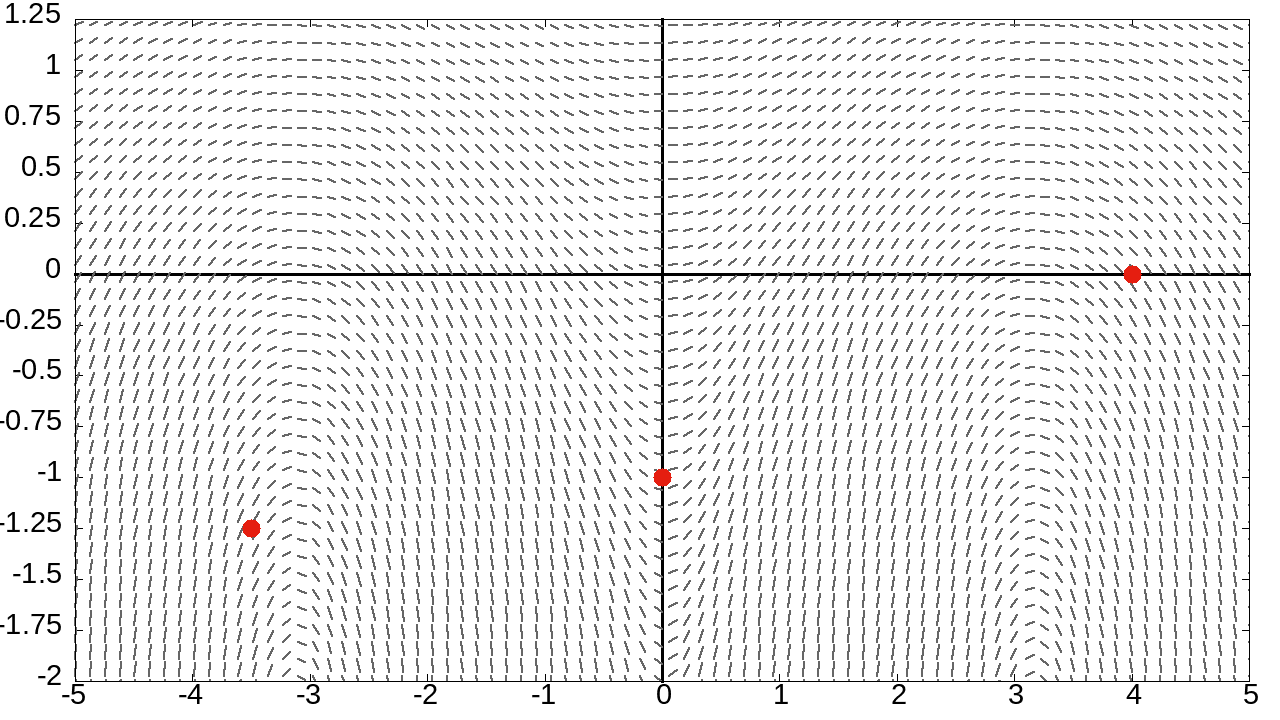
\includegraphics[width=0.95\textwidth]{slopefield.png}
\end{center}


\begin{enumerate}[label=(\alph*)]

\item Erklären Sie kurz, was man unter einer partikulären Lösung und einer Anfangsbedingung versteht. Wie unterscheidet sich diese von der allgemeinen Lösung?
 
\item Geben Sie einen Vektor an, der die Richtung des Richtungspfeils am Punkt $(\frac{3}{2}\pi, -\ln(3))$ darstellt!

\item Tragen Sie in der oberen Skizze für jede der mit einem Kreis dargestellten Anfangsbedinungen die partikuläre Lösung ein! 

\end{enumerate}

\newpage
\section* {Aufgabe 2}

Beim Addieren von Brüchen wird manchmal die folgende (im Allgemeinen falsche) Umformung angewandt:

\begin{align*}
&\frac{a}{c} + \frac{b}{d} = \frac{a+b}{c+d}\\
\end{align*}

\begin{enumerate}[label=(\alph*)]

\item Welchen Grundbereich hat das Tupel $(a, b, c, d)$ -- $\mathbb{N}^4$, $\mathbb{Z}^4$, $\mathbb{Q}^4$ oder $\mathbb{R}^4$? Warum?
\item Welche Bedingung muss gelten für $(a, b, c, d)$, damit obige Umformung definiert ist?
\item Sei $a=b=0$. Für welche Tupel $(a, b, c, d)$ ist die obige Umformung korrekt?
\item Sei nun $a \ne 0$, $b \ne 0$. Welche zusätzlichen Tupel $(a, b, c, d)$ ergeben sich? Geben Sie ein konkretes solches Tupel an!

\end{enumerate}

\newpage
\section* {Aufgabe 3}

Die Regel von l'Hôpital hilft beim Bestimmen von Grenzwerten und lautet:

$$\lim\limits_{x \to a} \frac{f(x)}{g(x)} = \lim\limits_{x \to a} \frac{f'(x)}{g'(x)} $$

\begin{enumerate}[label=(\alph*)]
\item Welche Voraussetzungen müssen gelten, damit obige Regel anwendbar ist?
\item Bestimmen Sie damit den Grenzwert $G_1 = \lim\limits_{x\to 0}\sin(x) \cdot x^{-1}$!
\item Bestimmen Sie damit den Grenzwert $G_2 = \lim\limits_{x\to\infty}\sqrt[\leftroot{-2}\uproot{2}x]{x}$!\\
(Hinweis: $\sqrt[\leftroot{-2}\uproot{2}x]{x} = x^{1/x}$. Betrachten Sie $\ln(G_2)$.)
\end{enumerate}

\newpage
\section* {Aufgabe 4}

Betrachtet werde die Differentialgleichung (DGL):

$$y^2 \cdot (y')^2 + y^2 = 1$$

\begin{enumerate}[label=(\alph*)]
\item Klassifizieren Sie diese DGL hinsichtlich Ordnung, Homogenität und Linearität!
\item Zeigen Sie, dass die allgemeine Lösung der DGL $y^2+(x-C)^2 = 1$ lautet!\\
(Hinweis: Trennung der Variablen, Substitution $u=y^2$ für das Integral über y)
\item Die allgemeine Lösung $\Phi(x,y,C)=0$ stellt eine Kurvenschar dar, deren Einhüllende ebenfalls Lösung sind. Die Einhüllenden $y(x)$ ergeben sich, indem man die beiden Gleichungen $\Phi(x,y,C) = 0 = \frac{\partial \Phi(x,y,C)}{\partial C}$ so umstellt, dass der Parameter $C$ eliminiert wird. Finden Sie diese Einhüllenden $y(x)$!
\end{enumerate}

Anmerkung: Bei den Lösungskurven handelt es sich um Kreise mit dem Radius 1, deren Mittelpunkte auf der Abzisse liegen.

\end{document}
